\chapter{Error probability and timeouts study} \label{chapter:errors}
\section{Introduction}
This annex has been written with the purpose to quantify the error probability that transcievers that implement the Network Mode standard can suffer, as well as to study the minimum timeout requirements. A proper analysis can lead to optimal values than enhance the performance without hurting the robustness of the standard.

% This document has been written with the purpose to quantify the error probability that transcievers that implement the Network Mode standard can suffer, and from there justify the chosen amount of retry attemps for a concrete application. Moreover, a general timeout definition is made, used later to provide the required minimum timeout for a concrete implementation of the standard.

\subsection{Scope}
This document establishes the minimum number of retries and the minimum timeout to achieve a successful Network Mode standard operation. It starts from generic explanations and equations to later focus on the Network Mode particular case. For both chapters there are, first, theoretical sections; and after a section that shows calculations for a concrete application.

This document is applicable to transcievers that implement the Network Mode standard in its totality. Numerical results given as examples are made for the Network Mode competition constraints; the reader should perform his own calculations if he brings the Network Mode standard to other scenarios.


\section{Error probability}

\subsection{Required number of retries}
The bit error rate (BER) can be understood as the expectancy for a bit, sent by a transmitter, to be flipped at the receiver side, by unit of time. To avoid time dependency this document makes use of bit error probability, defined as $p_{eb}$. If multiple bits are exchanged between a transmitter and a receiver, then the following holds:
\begin{equation}
	p_{eb} = \text{E} \left \{ \frac{ \text{\# erroneous bits}}{\text{\# total bits}}  \right \} = \frac{ \text{E} \left \{  \text{\# erroneous bits}  \right \} }{\text{\# total bits}} \ .
\end{equation}

The Network Mode standard defines how packets of bits are exchanged between nodes. Here, a packet is considered erroneous if at least one of its bits is incorrect. Then, the probability for a packet to have at least one error can be understood as a particular binomial distribution case in which the number of trials is equal to the number of trials in which the bit hasn't been flipped.
\begin{equation}
	P(x)|_{x=n} = \binom{n}{x} p^x \left( 1-p \right)^{n-x} = p^x \ .
\end{equation}
Where $p$ is the event probability, $n$ the number of trials and $x$ the number of trials for which the event occurs.

The probability for a packet to differ, at least by $1$ bit, with respect to the one at the transmitter side is defined as $p_{ep}$. For $N$ bits in a packet, with the bit error probability being $p_{eb}$, $p_{ep}$ is defined as $1$ minus the probability of having $N$ out of $N$ bits correct.
\begin{equation}
	p_{ep} = 1 - \left( 1 - p_{eb} \right)^N \ .
	\label{eq:pep}
\end{equation}

It's already conceived in the standard that some received packets may contain errors, and thus the packet can be resent, i.e., a retry is made from the transmitter side. The probability to fail after $T$ tries is named $p_{\text{fail}}$ and follows
\begin{equation}
	\begin{split}
		& p_{\text{fail}} = \left( p_{ep} \right)^T \\
		& p_{\text{fail}} = \left(  1 - \left( 1 - p_{eb} \right)^N
 \right)^T \\
	\end{split} \ .
\end{equation}
It's a goal of the standard to achieve a robust communication, which means the probability of failing at sending a certain packet of $N$ bits after $T$ tries should be lower than a desired threshold.
\begin{equation}
		p_{\text{fail}} = \left(  1 - \left( 1 - p_{eb} \right)^N   \right)^T < p_{\text{fail threshold}} \ .
\end{equation}
The number of packet bits $N$ is fixed by the defined packets, and $p_{eb}$ can be derived after link budget calculations. The fail probability $p_{\text{fail threshold}}$ is set to an arbitrary value. The unknown is the number of tries required, $T$, which can only take integer values equal or higher than $1$. Because the number inside the parenthesis must always be lower than $1$, $T$ must respect a minimum value.
\begin{equation}
	T > \frac{\ln \left( p_{\text{fail threshold}}  \right) }{\ln \left( 1 - \left( 1 - p_{eb} \right)^N \right) } \ .
	\label{eq:R}
\end{equation}
The number of retries is just
\begin{equation}
	R = T - 1 \ .
\end{equation}



\subsection{Bit error probability $p_{eb}$}
% LNA: https://wiki.iteadstudio.com/NRF24L01_with_PA_and_LNA_Module . Molt clau
RF modules manufacturers typically provide the expected bit error probability (usually named as BER) for a single received power. To solve \eqref{eq:R} for $T$, link budget calculations are required, and the calculated received power signal at the receiver end should be used to determine $p_{eb}$.

Complex equations could be used to express $p_{eb} \left( E_b/N_0 \right)$, where $E_b$ is the bit energy and $N_0$ is two times the noise added by the channel; but this job has already been done by \textcite{Luque2012}. In the paper, the authors study a Bluetooth system, which works with Gaussian frequency-shift keying (GFSK). The Network Mode proposed standard uses GFSK. The bit error probability depends on the modulation index $h$. The $p_{eb}$ is plotted against the $E_b/N_0$ (dB) ratio in \Cref{fig:Luque-GFSK-png}.
\begin{figure}[H] \centering
	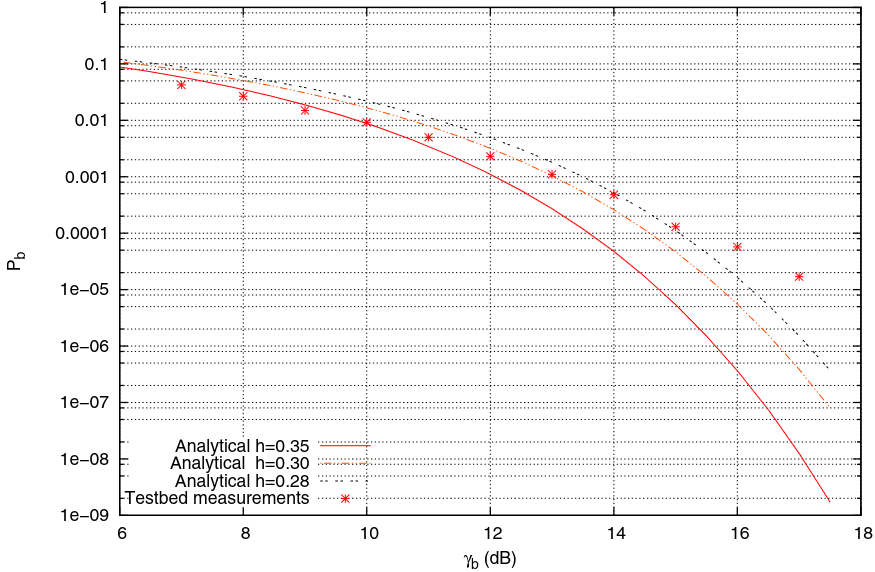
\includegraphics[width=0.8\textwidth]{Luque-GFSK.png}
	\caption{$p_{eb}$ as a function of $E_b/N_0$ (\SI{}{\dB}), from \textcite{Luque2012}}
	\label{fig:Luque-GFSK-png}
\end{figure}
The standard doesn't specify a concrete $h$ value. The testbed measurements will be used for future calculations because it's the worst case for large $E_b / N_0$ values and shows quite a linear trend in the logarithmic axes.

The number of symbols of a codification, named $M$, follows
\begin{equation}
	M = 2^{R_b/BW} \ ,
	\label{eq:Rb}
\end{equation}
where $BW$ is the bandwidth and $R_b$ the bandwidth efficiency. In GFSK there are only two symbols possible: $0$ or $1$. This means $R_b = BW$. 

The signal-to-noise ratio $SNR$ at the output of the receiver demodulator is defined in the paper as
\begin{equation}
	SNR = \frac{E_b}{N_0 \cdot BW \cdot T_b} \ ,
\end{equation}
where $T_b = \frac{1}{R_b}$ is the bit transmission period. Substituting \eqref{eq:Rb} leads to
\begin{equation}
	SNR = \frac{E_b}{N_0} \ ,
\end{equation}
for the particular GFSK case. By definition the receiver sensitivity is the power level for which a certain received signal leads to a certain BER, and this means
\begin{equation}
	SNR = \frac{E_b}{N_0} \left[ \SI{}{\dB} \right]  = P_{RX} \left[ \SI{}{\dB}\text{m} \right]   - \left( P_{RX\text{, sensitvity}} \left[ \SI{}{\dB}\text{m} \right] - P_{\text{offset}} \left[ \SI{}{\dB}\text{m} \right] \right)   \ ,
\end{equation}
% 
where $P_{\text{offset}}$ is the power difference between the noise floor and the sensitivity that has been specified for a certain BER smaller than $0.5$.

In order to find $P_{RX}$ link budget calculations are necessary. Assuming quite and ideal case with line of sight (LOS) and no ground reflections,
\begin{equation}
	\begin{split}
		P_{RX} \left[ \SI{}{\dB}\text{m} \right] =& P_{TX} \left[ \SI{}{\dB}\text{m} \right] +  G_{\text{antenna TX}} \left[ \SI{}{\dB} \right]  - 20 \log\left( \frac{4 \pi d}{\lambda} \right) \left[ \SI{}{\dB} \right] +   \\
												  &   G_{\text{antenna RX}} \left[ \SI{}{\dB} \right] -  G_{\text{losses}} \left[ \SI{}{\dB} \right]  \\
	\end{split} \ .
	\label{eq:link}
\end{equation}
Where $d$ is the distance between antennas, and the gain that antennas can offer and extra possible losses has been considered.


Using the previous definitions \eqref{eq:R} can be solved. As a summary, $P_{RX}$ should be calculated from the link budget, and $P_{RX\text{, sensititivy}}$ can be either calculated from LNA noise figure (NF) and input thermal noise, or taken from the receiver manufacturer specifications. Then, if $P_{\text{offset}}$ is known it's straightforward to get $\frac{E_b}{N_0}$. Next, a plot such as the one in \Cref{fig:Luque-GFSK-png} can be used to get the bit error probability, $p_{eb}$. Finally, this value is substituted in \eqref{eq:R} together with the $N$ bits of the packet and an arbitrary $p_{\text{fail threshold}}$,





\subsection{Numerical example for the NM competition scenario}
The purpose of this section is to provide some application-dependant orientative numbers to solve for $T$.


\subsubsection{DATA packet, neighbour distance} \label{sub:data1}
First, for the link budget it's taken into account that nRF24 output power is set to \SI{-6}{\dB}m. The nRF24l01 comes, often, soldered in a board together with a \SI{20}{\dB} power amplifier (PA), leading to a transmitted power of \SI{14}{\dB}m. Moreover, it contains a low noise amplifier (LNA) that provides \SI{10}{\dB}. The sensitivities given by the manufacturer are referenced to the LNA output, meaning that at the LNA input they are \SI{10}{\dB} lower. 

Both the transmitter and the receiver antennas show the same gain: $G_{\text{antenna RX}} = G_{\text{antenna TX}} = \SI{2}{\dB}$. $G_{\text{losses}}$ is set to \SI{12}{\dB} to account for the ground reflection effect and the fact that, after some measurements, it was seen that the output power was a few \SI{}{\dB} shy of the one specified by the manufacturer.

It's assumed $3$ transcievers will be placed at the \SI{260}{\m} Campus Nord side, meaning the worst case distance between transcievers is $d = \SI{130}{\m}$. Up to $4$ devices are expected on the short side, with the corner device being taken into account. The central frequency of operation must be between \SI{2.4}{\GHz} and \SI{2.525}{\GHz}. Channel 27 was chosen because of interference reasons, meaning the central frequency is \SI{2.427}{\GHz}.

With all the considered values \eqref{eq:link} is solved.
\begin{equation}
	\begin{split}
		& P_{RX} \left[ \SI{}{\dB}\text{m} \right] = \SI{14}{\dB}\text{m} +  \SI{2}{\dB}  - 20 \log\left( \frac{4 \pi \SI{130}{\m}}{\frac{\SI{3e8}{\m\per\s}}{\SI{2.427}{\GHz}}} \right) \left[ \SI{}{\dB} \right] + \SI{2}{\dB} - \SI{12}{\dB} \\
		& P_{RX} = - \SI{76.42}{\dB}\text{m}
	\end{split} \ .
\end{equation}
For the nRF24, at $250$kbps the sensitivity that achieves $p_{eb} = \SI{1e-3}{}$ is $- \SI{94}{\dB}\text{m} - \SI{10}{\dB}\text{m} = - \SI{104}{\dB}\text{m}$. The difference between the received power at the LNA input and the mentioned sensitivity is $- \SI{76.42}{\dB}\text{m} - \left( - \SI{104}{\dB}\text{m} \right) = \SI{27.58}{\dB}$.

Now, from \Cref{fig:Luque-GFSK-png} and testbed measurements it's derived that to get $p_{eb} = \SI{1e-3}{}$, $\frac{E_b}{N_0} = \SI{13}{\dB}$. If there's a \SI{27.58}{\dB} difference between the received power and the sensitivity for which $p_{eb} = \SI{1e-3}{}$, then $p_{eb}$ is obtained by looking at $\frac{E_b}{N_0} \approx \SI{40}{\dB}$. 

The testbed measurements plot is quite linear in a logarithmic scale, with an approximate slope of $\approx 3.5$ decades for every \SI{10}{\dB} increase in $\frac{E_b}{N_0}$. Thus, in this numeric case $p_{eb} \approx \SI{1e-13}{}$.


The DATA packet defined in the protocol requires $30$ bytes plus $7$ bits. This payload is fitted inside the nRF24 packet. This means a preamble of $1$ byte, an address of up to $5$ bytes, a packet control field of $9$ bits and a CRC of up to $2$ bytes are also required. This adds up to
\begin{equation}
	N = \left( 1 + 5 + 2  + 30 \right)  \text{ bytes} \times \frac{8 \text{ bits}}{1 \text{ byte}} + 9 \text{ bits} + 7 \text{ bits} = 320 \text{ bits} \ .
\end{equation}
Substituting the $N$ number of bits and the bit error probability $p_{eb}$ into \eqref{eq:pep} leads to the following $p_{ep}$ packet error:
\begin{equation}
	\begin{split}
		& p_{ep} = 1 - \left( 1 - p_{eb} \right)^N \\
		& p_{ep} = 1 - \left( 1 - \SI{1e-13}{} \right)^{320} \\
		& p_{ep} = \SI{3.20e-11}{}
	\end{split} \ .
\end{equation}
A failure threshold of $p_{\text{fail threshold}} = \SI{1e-16}{}$ is imposed and $T$ is found using \eqref{eq:R}.
\begin{equation}
	\begin{split}
		& T > \frac{\ln \left( p_{\text{fail threshold}}  \right) }{\ln \left( 1 - \left( 1 - p_{eb} \right)^N \right) } \\
		& T > \frac{\ln \left( \SI{1e-16}{} \right) }{\ln \left( 1 - \left( 1 - \SI{1e-13}{} \right)^{320} \right) } \\
		& T > 1.525 \\
		& T \rightarrow 2 \\
	\end{split} \ .
\end{equation}
This means that the number of retries is just
\begin{equation}
	R = 1 \ ,
\end{equation}
due to the low probability of getting a packet wrong. The fact that the \SI{250}{}kbps datarate is set means the sensitivity is very low and leads to a very robust communication for the distances the application requires, according to theoretical calculations.



\subsubsection{DATA packet, maximum distance} \label{sub:data3}
The previous case considered the distance between transmitter and receiver was just $d = \SI{130}{\m}$. Although this is expected to be the most common case, the low sensitivity makes it possible to send data at higher distances. Here, $d = \SI{260}{\m}$, which is the maximum line of sight (LOS) distance expected, is taken.

From \eqref{eq:link}, it's enough to calculate the received power decrease because of the distance increase.
\begin{equation}
	\begin{split}
	&	\Delta P_{RX} = - 20 \log \left( d_{\text{current}} \right)  + 20 \log \left( d_{\text{previous}} \right)  \\
	&	\Delta P_{RX} = - 20 \log \left( \SI{260}{\m} \right)  + 20 \log \left( \SI{130}{\m} \right)  \\
	&	\Delta P_{RX} = - \SI{6.02}{\dB}
	\end{split} \ .
\end{equation}
Thus,
\begin{equation}
	\begin{split}
		& P_{RX} = P_{RX \text{, previous}} + \Delta P_{RX} \\
		& P_{RX} = - \SI{76.42}{\dB}\text{m} - \SI{6.02}{\dB} \\
		& P_{RX} = - \SI{82.44}{\dB}\text{m} \\
	\end{split} \ .
\end{equation}
In this case, the difference of the received power with respect to the senstivity level is $\SI{-82.44}{\dB}\text{m} - \left( - \SI{104}{\dB}\text{m} \right) = \SI{21.56}{\dB}$. Adding up the \SI{13}{\dB}, the \Cref{fig:Luque-GFSK-png} must be analyzed at \SI{34.56}{\dB}. In this case, by extrapolating the testbed measurements plot a safe value to take is
\begin{equation}
	p_{eb} = \SI{1e-11}{} \ .
\end{equation}
Considering the $N = 320$ bits of the DATA packet, the packet error probability is:
\begin{equation}
	\begin{split}
		& p_{ep} = 1 - \left( 1 - p_{eb} \right)^N \\
		& p_{ep} = 1 - \left( 1 - \SI{1e-11}{} \right)^{320} \\
		& p_{ep} = \SI{3.2e-9}{}
	\end{split} \ .
\end{equation}
The difference with the previous case is around $4$ orders of magnitude. Again, a failure threshold of $p_{\text{fail threshold}} = \SI{1e-16}{}$ is imposed and $T$ is found using \eqref{eq:R}.
\begin{equation}
	\begin{split}
		& T > \frac{\ln \left( p_{\text{fail threshold}}  \right) }{\ln \left( 1 - \left( 1 - p_{eb} \right)^N \right) } \\
		& T > \frac{\ln \left( \SI{1e-16}{} \right) }{\ln \left( 1 - \left( 1 - \SI{1e-11}{} \right)^{320} \right) } \\
		& T > 1.88 \\
		& T \rightarrow 3 \\
	\end{split} \ .
\end{equation}
Just to be safe, as the result is close to its ceiling integer, the result has been approximated to $3$ tries. This means that the number of retries must be
\begin{equation}
	R = 2 \ .
\end{equation}
Thanks to the exponential dependence of $p_{ep}$ on the number of tries $T$ the $4$ orders of magnitude between the two cases don't require a tries difference.



\subsubsection{TOKEN packet, neighbour distance} \label{sub:token1}
The two previous cases detailed in subsections \ref{sub:data1} and \ref{sub:data3} refer to the DATA packet, which is the largest packet specified by the standard. However, the TOKEN packet should also be considered. As mentioned in the standard, a transmitter needs to make sure if a node is available of not. The TOKEN packet contains a variable part of \SI{3}{} bits, larger than the \SI{2}{} bits of the HELLO RESPONSE packet. The TOKEN packet is analyzed because it's the largest of the two.

Thanks to previous calculations the $P_{RX}$ power are already known. Changes appear, now, at the packet number of bits, $N$.
\begin{equation}
	N = \left( 1 + 5 + 2  \right)  \text{ bytes} \times \frac{8 \text{ bits}}{1 \text{ byte}} + 9 \text{ bits} + 3 \text{ bits} = 67 \text{ bits} \ .
\end{equation}


For the neighbour distance
\begin{equation}
		P_{RX} = - \SI{76.42}{\dB}\text{m} \ .
\end{equation}
Recall this lead to
\begin{equation}
	p_{eb} = \SI{1e-13}{} \ .
\end{equation}
Considering the $N = 67$ bits of the TOKEN packet, the packet error probability is:
\begin{equation}
	\begin{split}
		& p_{ep} = 1 - \left( 1 - p_{eb} \right)^N \\
		& p_{ep} = 1 - \left( 1 - \SI{1e-13}{} \right)^{67} \\
		& p_{ep} = \SI{6.70e-12}{}
	\end{split} \ .
\end{equation}
In this case, the packet failure threshold is decreased by two orders of magnitude with respect to the DATA packet, i.e., $p_{\text{fail threshold}} = \SI{1e-18}{}$. This number is arbitrary, but the authors want to emphasize the importance of sending the TOKEN packet properly. \eqref{eq:R} is solved for $T$.
\begin{equation}
	\begin{split}
		& T > \frac{\ln \left( p_{\text{fail threshold}}  \right) }{\ln \left( 1 - \left( 1 - p_{eb} \right)^N \right) } \\
		& T > \frac{\ln \left( \SI{1e-18}{} \right) }{\ln \left( 1 - \left( 1 - \SI{1e-13}{} \right)^{67} \right) } \\
		& T > 1.610 \\
		& T \rightarrow 2 \\
	\end{split} \ .
\end{equation}
On one hand, the threshold has been decreased; on the other the number of bits $N$ is lower. This means that the number of retries must be just $1$ for the neighbour distance.
\begin{equation}
	R = 1 \ .
\end{equation}



\subsubsection{TOKEN packet, 3 nodes distance}
The main difference with respect to subsection \ref{sub:token1} is that now $P_{RX} = \SI{-82.44}{\dB}$m, which means
\begin{equation}
	p_{eb} = \SI{1e-11}{} \ .
\end{equation}
Recall the defined TOKEN packet contains $N = 67$ bits. Then,
\begin{equation}
	\begin{split}
		& p_{ep} = 1 - \left( 1 - p_{eb} \right)^N \\
		& p_{ep} = 1 - \left( 1 - \SI{1e-11}{} \right)^{67} \\
		& p_{ep} = \SI{6.70e-10}{}
	\end{split} \ .
\end{equation}
There's been a $2$ orders of magnitude increase in $p_{ep}$ with respect to subsection \ref{sub:token1}. Again, the packed failure threshold is set to $p_{\text{fail threshold}} = \SI{1e-18}{}$. \eqref{eq:R} is solved for $T$.
\begin{equation}
	\begin{split}
		& T > \frac{\ln \left( p_{\text{fail threshold}}  \right) }{\ln \left( 1 - \left( 1 - p_{eb} \right)^N \right) } \\
		& T > \frac{\ln \left( \SI{1e-18}{} \right) }{\ln \left( 1 - \left( 1 - \SI{1e-11}{} \right)^{67} \right) } \\
		& T > 1.962 \\
		& T \rightarrow 3 \\
	\end{split} \ .
\end{equation}
On one hand, the threshold has been decreased; on the other the number of bits $N$ is lower. Again, because the value is very close to its ceiling integer the number of tries has been made $3$.
\begin{equation}
	R = 2 \ .
\end{equation}


\subsubsection{Summary}
The obtained results are summarized below:
\begin{table}[H]
	\centering
	\begin{tabular}{|r|r|r||r|r|} \hline
		Packet & Distance (\SI{}{\m}) & $p_{\text{fail threshold}}$ & Number of tries $T$ & Number of retries $R$ \\ \hline \hline
		DATA & \SI{130}{\m} & \SI{1e-16}{} & $2$ & $1$ \\ \hline
		DATA & \SI{260}{\m} & \SI{1e-16}{} & $3$ & $2$ \\ \hline
		TOKEN & \SI{130}{\m} & \SI{1e-18}{} & $2$ & $1$ \\ \hline
		TOKEN & \SI{260}{\m} & \SI{1e-18}{} & $3$ & $2$ \\ \hline
	\end{tabular}
	\caption{Number of tries and retries, summary}
	\label{tab:label}
\end{table}

In conclusion, it's been justified that for both the DATA and TOKEN packets a total of $T=3$ tries, i.e., $R=2$ retries are required, to meet the set thresholds for the \SI{260}{\m} distance.









\section{Timeouts}

\subsection{Theoretical explanation}
As important as the number of tries and retries are, it's also critical to determine the timeouts required for a transmitter to switch to a receiver and wait for acknowledgements (ACKs) from potential receivers that switch to transmitters after they have received a package.

It should be made clear that the timeout is defined here as the maximum loop time in which a transmitter will be stuck waiting for an acknowledgement signal. Too small, and there won't be time to receive the ACK. Too large, and the transmitter will waste time waiting for no signal. This means there's an optimal timeout. It's the aim of this chapter to find it. 

Moreover, it can be noticed from the given definition that the timeout is independent of the package length that has been sent. It can, however, be made dependant on the ACK packet length.

The timeout at the receiver side must meet the following equation.
\begin{equation}
	\begin{split}
	& t_{\text{timeout}} \geq t_{\text{air}} + t_{\mu \text{C, RX}} + t_{\text{RTAD}} + t_{\text{RX}} + t_{\text{air}} + t_{\mu \text{C, TX}} + t_{\text{RTAD}}  \\
	& t_{\text{timeout}} \geq 2 t_{\text{air}} + t_{\text{RX}} + \left(  t_{\mu \text{C, RX}} + t_{\mu \text{C, TX}} \right) +  2 t_{\text{RTAD}}  \\
	\end{split} \ .
	\label{eq:timeout}
\end{equation}
Where $t_{\text{air}}$ is the amount of time the last bit sent by the transmitter TX is received by the receiver TX, $t_{\text{TX}}$ is the duration of time the receiver requires to send the ACK packet, $t_{\mu \text{C, RX}}$ and $t_{\mu \text{C, TX}}$ are the required times at the RF modules microcontrollers to interpret the received packet and take a decision from there, and $t_{\text{RTAD}}$ is the radio turn around delay, which is the time a transciever requires to switch from transmitter to receiver or viceversa.


The packets are sent at the speed of light, meaning $t_{\text{air}}$ is
\begin{equation}
	t_{\text{air}} = \frac{d}{c} \ .
\end{equation}
Where $d$ is the distance between transmitter and receiver, and $c$ is the speed of light $c \approx \SI{3e8}{\m\per\s}$.

The time required by the receiver to send the ACK packet, $t_{\text{RX}}$, is 
\begin{equation}
	t_{\text{RX}} = \frac{\text{Packet size} \left[\text{bits} \right]}{ \text{Datarate} \left[\frac{\text{bits}}{\text{s}} \right]}  \ .
\end{equation}
The time spent spent at the RF module microcontroller, $t_{\mu \text{C}}$, is proportional to the clock periods to fetch, decode and execute the required instructions to process the message and take a decision. This depends on the integrated circuit internal operation and clock frequency.

The $t_{\text{RTAD}}$ time is typically specified by the RF module manufacturer.



\subsection{Numerical example for the NM competition scenario}
Once the timeout equation \eqref{eq:timeout} has been specified, numerical values can be substituted to calculate the timeout required for a real application.

The maximum expected line of sight communication distance during the NM competition is $d = \SI{260}{\m}$. Thus,
\begin{equation}
	\begin{split}
	& t_{\text{air}} = \frac{d}{c} \\
	& t_{\text{air}} = \frac{\SI{260}{\m}}{\SI{3e8}{\m\per\s}} \\
	& t_{\text{air}} = \SI{86.67}{\ns}
	\end{split} \ .
\end{equation}
The time required to transmit an ACK package depends on its length. Although all packages defined in the standard have very similar lengths, the largest one is considered here. It's the DATA ACK packet, that shares the length with the HELLO RESPONSE packet. Both have $2$ bits of information plus the fixed bytes and bits of the nRF24.
\begin{equation}
	N = \left( 1 + 5 + 2  \right)  \text{ bytes} \times \frac{8 \text{ bits}}{1 \text{ byte}} + 9 \text{ bits} + 2 \text{ bits} = 66 \text{ bits} \ .
\end{equation}
The standard specifies $\text{Datarate} = 250$ kbps.
\begin{equation}
	t_{\text{RX}} = \frac{66 \left[\text{bits} \right]}{ \SI{250e3}{} \left[\frac{\text{bits}}{\text{s}} \right]}  = \SI{264}{\us} \ .
\end{equation}
The $t_{\mu \text{C}}$ times are not specified by Nordic, the nRF24 manufacturer, and one may suspect these times are be already included in $t_{\text{RTAD}}$. In case of doubt, the following assumption is made:
\begin{equation}
	t_{\mu \text{C, RX}} = t_{\mu \text{C, TX}} = t_{\mu \text{RTAD}} \ .
\end{equation}
According to the nRF24 specifications
\begin{equation}  
	t_{\text{RTAD}} = \SI{130}{\us} \ .
\end{equation}
Finally, numerical values are plugged into \eqref{eq:timeout}.
\begin{equation}
	\begin{split}
	& t_{\text{timeout}} \geq 2 t_{\text{air}} + t_{\text{RX}} + \left(  t_{\mu \text{C, RX}} + t_{\mu \text{C, TX}} \right) +  2 t_{\text{RTAD}}  \\
	& t_{\text{timeout}} \geq 2 \times \SI{86.67}{\ns} + \SI{264}{\us} + 2 \times \SI{130}{\us} +  2 \times \SI{130}{\us} \\
	& t_{\text{timeout}} \geq  \SI{784}{\us}
	\end{split} \ .
\end{equation}
This is the minimum time required between two transmissions at the transmitter side. There's a high chance the nRF24 already implements some of the timeout sumands. Anyways, the communication should work fine if the above timeout is imposed to wait for all the possible responses.
















